% appendices/pen-test.tex

\chapter{Detailed Peneteration Testing and Security Ecaluation}
\label{app:pen_test}

% --------------------------------------------------

\section*{Test 1 --- \texttt{/health} endpoint exposure}

\begin{figure}[h]
    \centering
    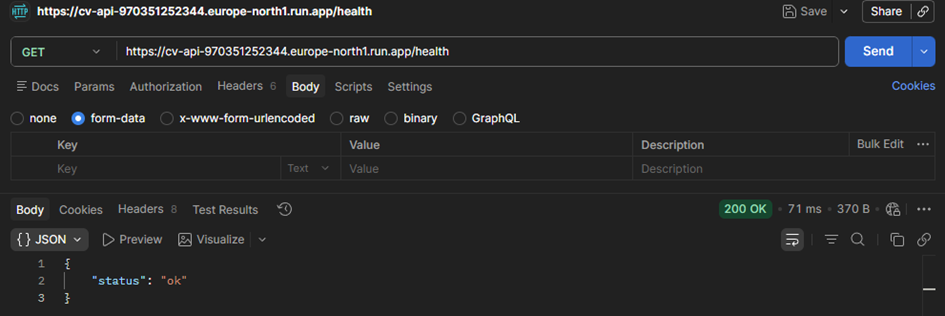
\includegraphics[width=\textwidth]{figures/images/chapter-9/pen-test/health-endpoint-exposure.png}
    \caption{Response from the public \texttt{/health} endpoint}
\end{figure}

\noindent \textbf{Test case:} Public health endpoint inspection

\noindent \textbf{Endpoint:} \texttt{GET /health}

\noindent \textbf{What was sent:} A simple \texttt{GET} request.

\noindent \textbf{Expected result:} A minimal status response without unnecessary internal information.

\noindent \textbf{Actual result:} The endpoint returned \texttt{200 OK} with the minimal JSON response \texttt{\{"status": "ok"\}}. No internal system details, debug data, or sensitive information were exposed.

\noindent \textbf{Assessment:} Worked as expected. The endpoint exposes only minimal health status information and does not appear to leak unnecessary internal data.

% --------------------------------------------------

\section*{Test 1 --- Valid \texttt{/api/detect} request}

\begin{figure}[H]
    \centering
    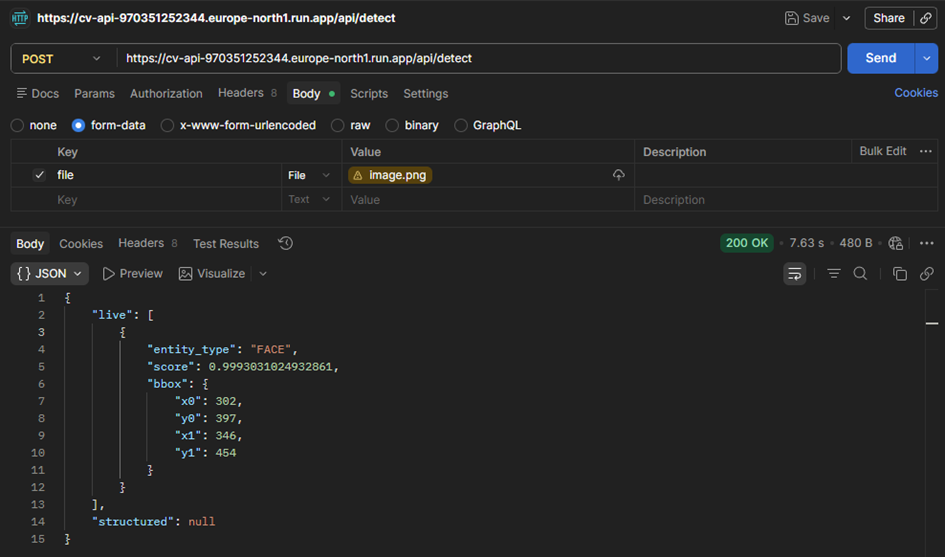
\includegraphics[width=\textwidth]{figures/images/chapter-9/pen-test/valid-api-detect-request.png}
    \caption{Response from a valid request to \texttt{/api/detect}}
\end{figure}

\noindent \textbf{Test case:} Valid image upload to \texttt{/api/detect} 

\noindent \textbf{Endpoint:} \texttt{POST /api/detect} 

\noindent \textbf{What was sent:} A normal image file using multipart form-data. 

\noindent \textbf{Expected result:} The API should return \texttt{200 OK} with detection results. 

\noindent \textbf{Actual result:} The API returned \texttt{200 OK}. The response contained detection output, including \texttt{entity\_type: "FACE"}, a confidence score, and bounding box coordinates. 

\noindent \textbf{Assessment:} Worked as expected. 

% --------------------------------------------------

\section*{Test 2 --- Invalid file disguised as image}

\begin{figure}[H]
    \centering
    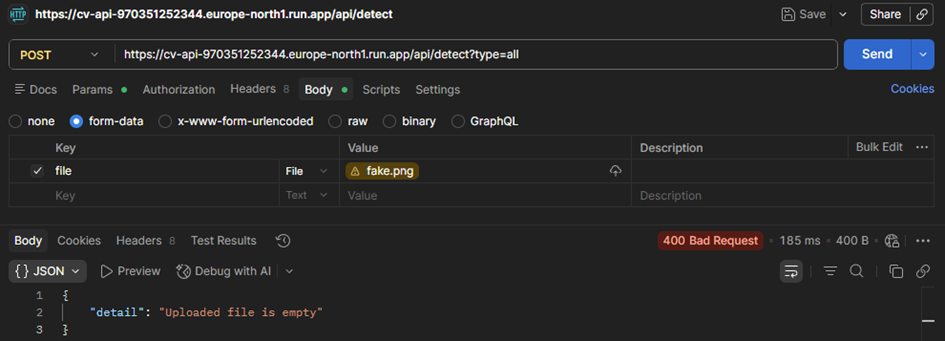
\includegraphics[width=\textwidth]{figures/images/chapter-9/pen-test/fake-image-test.png}
    \caption{Response from invalid file upload to \texttt{/api/detect}}
\end{figure}

\noindent \textbf{Test case:} Invalid file disguised as image 

\noindent \textbf{Endpoint:} \texttt{POST /api/detect} 

\noindent \textbf{What was sent:} An empty text file renamed to \texttt{.jpg} and uploaded as multipart form-data. 

\noindent \textbf{Expected result:} The API should reject the file without crashing and return an appropriate client error response. 

\noindent \textbf{Actual result:} The API returned \texttt{400 Bad Request} with the message \texttt{"Uploaded file is empty"}. 

\noindent \textbf{Assessment:} Worked as expected. The invalid input was handled safely, and the API returned a proper client-side error. 

% --------------------------------------------------

\section*{Test 4 --- Invalid JSON in \texttt{/api/redact}}

\begin{figure}[H]
    \centering
    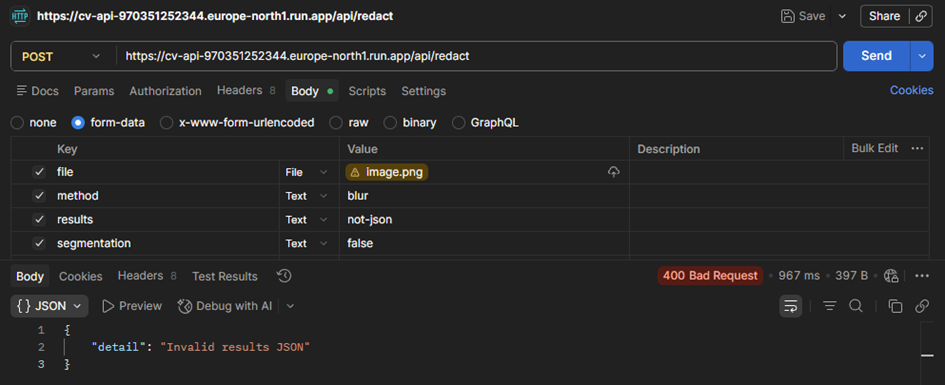
\includegraphics[width=\textwidth]{figures/images/chapter-9/pen-test/redact-invalid-json.png}
    \caption{Response from invalid JSON input to \texttt{/api/redact}}
\end{figure}

\noindent \textbf{Test case:} Invalid JSON in results for \texttt{/api/redact} 

\noindent \textbf{Endpoint:} \texttt{POST /api/redact} 

\noindent \textbf{What was sent:} A valid image, \texttt{method=blur}, \texttt{results=not-json}, and \texttt{segmentation=false}. 

\noindent \textbf{Expected result:} The API should reject the request with a controlled error. 

\noindent \textbf{Actual result:} The API returned \texttt{400 Bad Request} with the message \texttt{"Invalid results JSON"}. 

\noindent \textbf{Assessment:} Worked as expected. The invalid input was handled safely, and the API returned a proper client-side error without crashing. 

% --------------------------------------------------

\section*{Test 6 --- Invalid method in \texttt{/api/redact}}

\begin{figure}[H]
    \centering
    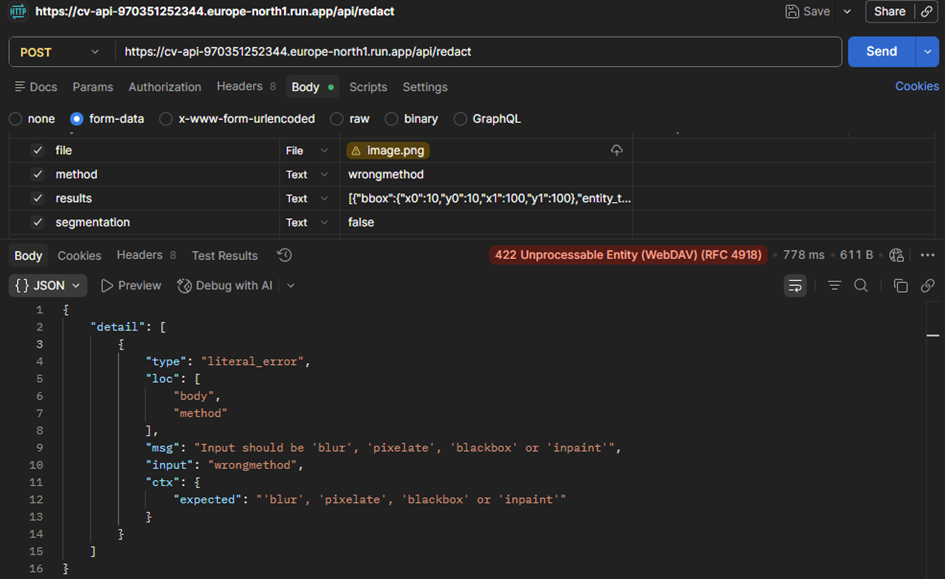
\includegraphics[width=\textwidth]{figures/images/chapter-9/pen-test/invalid-method-redact.png}
    \caption{Response from unsupported method input to \texttt{/api/redact}}
\end{figure}

\noindent \textbf{Test case:} Unsupported redaction method

\noindent \textbf{Endpoint:} \texttt{POST /api/redact}

\noindent \textbf{What was sent:} A valid request with a valid image and results payload, but with \texttt{method=wrongmethod}.

\noindent \textbf{Expected result:} The API should reject the request with a validation error.

\noindent \textbf{Actual result:} The API returned \texttt{422 Unprocessable Entity} with a validation message stating that the input should be \texttt{"blur"}, \texttt{"pixelate"}, \texttt{"blackbox"}, or \texttt{"inpaint"}.

\noindent \textbf{Assessment:} Worked as expected. The invalid method was blocked correctly, and the API returned a controlled validation error without crashing.

% --------------------------------------------------

\section*{Test 7 --- Extreme coordinates in \texttt{/api/redact}}

\begin{figure}[H]
    \centering
    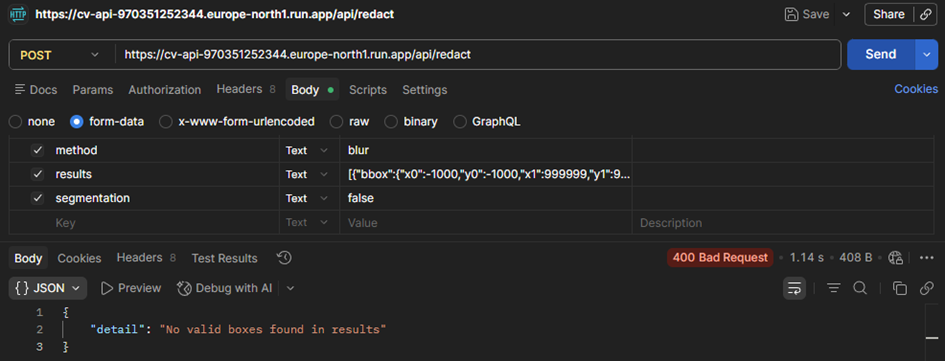
\includegraphics[width=\textwidth]{figures/images/chapter-9/pen-test/extreme-coordinates-redact.png}
    \caption{Response from extreme bounding box coordinates sent to \texttt{/api/redact}}
\end{figure}

\noindent \textbf{Test case:} Extreme bounding box coordinates

\noindent \textbf{Endpoint:} \texttt{POST /api/redact}

\noindent \textbf{What was sent:} A request with very large and negative bounding box coordinates in \texttt{results}: \texttt{[{"bbox":{"x0":-1000,"y0":-1000,"x1":999999,"y1":999999},"entity\_type":"FACE"}]}

\noindent \textbf{Expected result:} The API should handle the request safely without crashing.

\noindent \textbf{Actual result:} The API returned \texttt{400 Bad Request} with the message \texttt{"No valid boxes found in results"}.

\noindent \textbf{Assessment:} Worked as expected. The invalid bounding box coordinates were rejected safely, and the API returned a controlled client-side error without crashing.

% --------------------------------------------------

\section*{Test 10 --- Empty results list on \texttt{/api/redact}}

\begin{figure}[H]
    \centering
    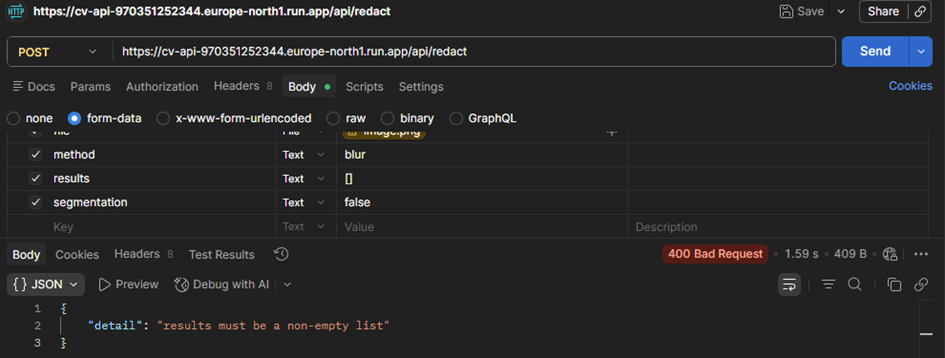
\includegraphics[width=\textwidth]{figures/images/chapter-9/pen-test/empty-results-redact.png}
    \caption{Response from empty \texttt{results} list sent to \texttt{/api/redact}}
\end{figure}

\noindent \textbf{Test case:} Empty results list in \texttt{/api/redact}

\noindent \textbf{Endpoint:} \texttt{POST /api/redact}

\noindent \textbf{What was sent:} A valid image, a valid method, and \texttt{results=[]}.

\noindent \textbf{Expected result:} The API should reject the request with a controlled validation error.

\noindent \textbf{Actual result:} The API returned \texttt{400 Bad Request} with the message \texttt{"results must be a non-empty list"}.

\noindent \textbf{Assessment:} Worked as expected. The empty \texttt{results} list was rejected correctly, and the API returned a controlled client-side error without crashing.

% --------------------------------------------------

\section*{Test 11 --- Malformed results structure on \texttt{/api/redact}}

\begin{figure}[H]
    \centering
    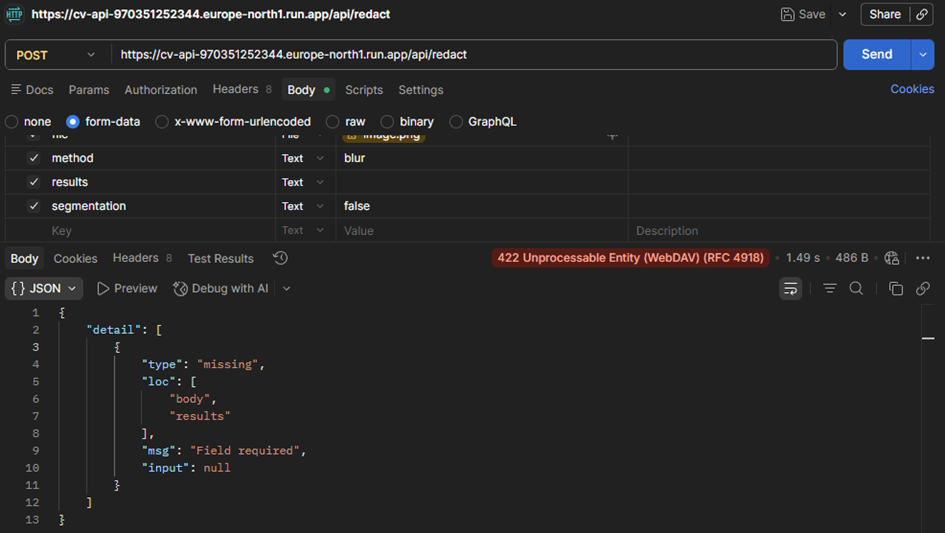
\includegraphics[width=\textwidth]{figures/images/chapter-9/pen-test/malformed-results-redact.png}
    \caption{Response from malformed \texttt{results} input sent to \texttt{/api/redact}}
\end{figure}

\noindent \textbf{Test case:} Malformed results structure in \texttt{/api/redact}

\noindent \textbf{Endpoint:} \texttt{POST /api/redact}

\noindent \textbf{What was sent:} A valid image and valid method, but the \texttt{results} field was malformed and did not contain the required structure. [{"foo":"bar"}]

\noindent \textbf{Expected result:} The API should reject the request or ignore invalid entries safely.

\noindent \textbf{Actual result:} The API returned \texttt{422 Unprocessable Entity} with a validation error stating that the \texttt{results} field was required.

\noindent \textbf{Assessment:} Worked as expected. The malformed input was handled safely, and the API rejected the request with a controlled validation error.

% --------------------------------------------------

\section*{Test 13 --- Many boxes in \texttt{/api/redact}}

\begin{figure}[H]
    \centering
    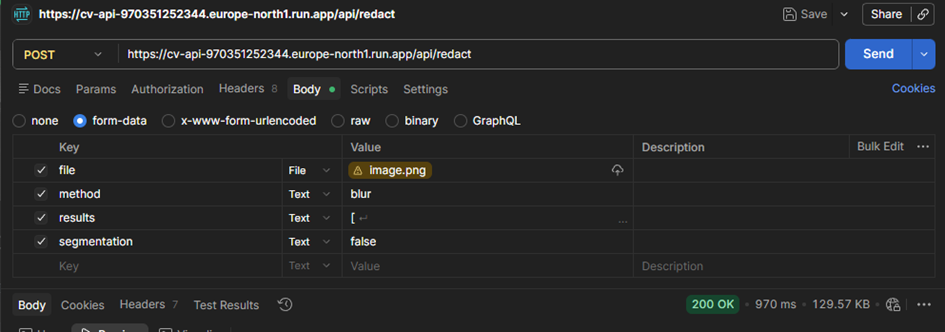
\includegraphics[width=\textwidth]{figures/images/chapter-9/pen-test/many-boxes-redact.png}
    \caption{Response from a \texttt{/api/redact} request with many bounding boxes}
\end{figure}

\noindent \textbf{Test case:} Large number of boxes in \texttt{/api/redact}

\noindent \textbf{Endpoint:} \texttt{POST /api/redact}

\noindent \textbf{What was sent:} A request containing many bounding boxes in the \texttt{results} field. The full payload is not visible in the screenshot because the Postman UI truncates long field values.

\noindent \textbf{Expected result:} The API should remain stable and either complete the request or fail in a controlled way.

\noindent \textbf{Actual result:} The API returned \texttt{200 OK} after approximately \texttt{970 ms}. The request completed successfully and returned a response body of approximately \texttt{129.57 kB}.

\noindent \textbf{Assessment:} Worked as expected. The endpoint remained stable under heavier input and completed the request successfully.

% --------------------------------------------------

\section*{Test 14 --- Invalid query parameters on \texttt{/api/detect}}

\begin{figure}[H]
    \centering
    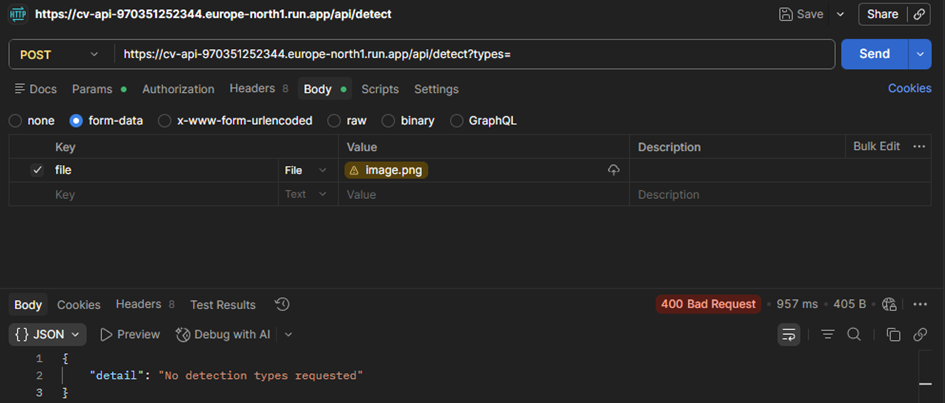
\includegraphics[width=\textwidth]{figures/images/chapter-9/pen-test/invalid-query-parameters-detect.png}
    \caption{Response from invalid query parameters sent to \texttt{/api/detect}}
\end{figure}

\noindent \textbf{Test case:} Invalid query parameters in \texttt{/api/detect}

\noindent \textbf{Endpoint:} \texttt{POST /api/detect}

\noindent \textbf{What was sent:} A request with an empty \texttt{types} query parameter value, shown as \texttt{/api/detect?types=}.

\noindent \textbf{Expected result:} The API should reject invalid parameter combinations safely.

\noindent \textbf{Actual result:} The API returned \texttt{400 Bad Request} with the message \texttt{"No detection types requested"}.

\noindent \textbf{Assessment:} Worked as expected. The invalid query parameter value was handled safely, and the API returned a controlled client-side error without crashing.

% --------------------------------------------------

\section*{Test 23 --- Very large request body / oversized file}

\begin{figure}[h]
    \centering
    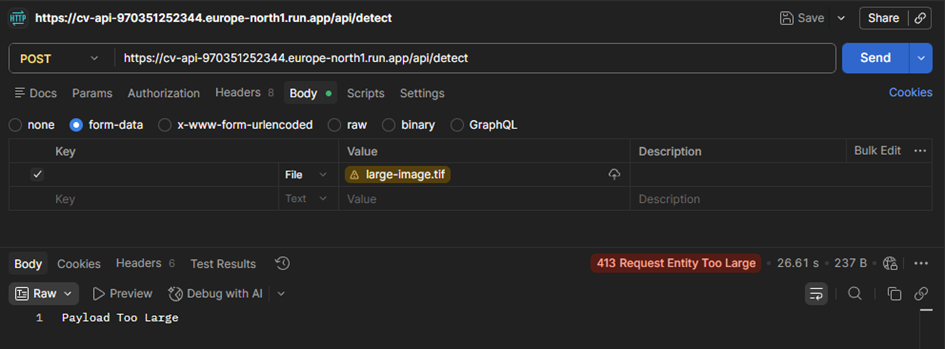
\includegraphics[width=\textwidth]{figures/images/chapter-9/pen-test/oversized-file-detect.png}
    \caption{Response from an oversized file upload sent to \texttt{/api/detect}}
\end{figure}

\noindent \textbf{Test case:} Oversized file upload

\noindent \textbf{Endpoint:} \texttt{POST /api/detect}

\noindent \textbf{What was sent:} A very large image file, shown as \texttt{large-image.tif}.

\noindent \textbf{Expected result:} The API should remain stable and either process the file or fail in a controlled way.

\noindent \textbf{Actual result:} The API returned \texttt{413 Request Entity Too Large} with the message \texttt{Payload Too Large}. The response was returned after approximately \texttt{26.61 s}, so the request was rejected in a controlled way rather than timing out or crashing.

\noindent \textbf{Assessment:} Worked as expected. The oversized upload was handled safely with a controlled error response. However, the response time was relatively high, so upload rejection could potentially be made faster depending on where size validation is enforced.

% --------------------------------------------------



% --------------------------------------------------

\section*{Test 8 --- Browser storage inspection}

\begin{figure}[H]
    \centering
    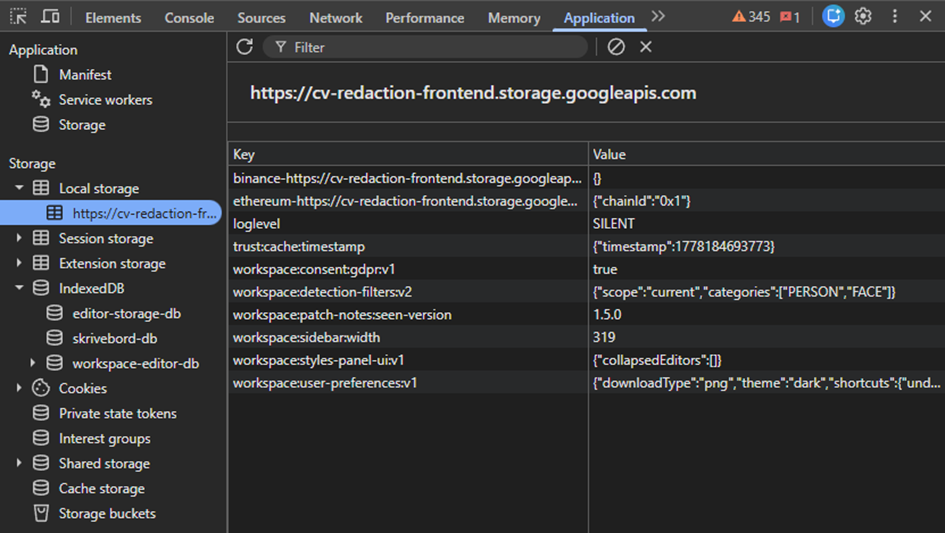
\includegraphics[width=\textwidth]{figures/images/chapter-9/pen-test/browser-storage-inspection.png}
    \caption{Local browser storage entries for the frontend application}
\end{figure}

\noindent \textbf{Test case:} Client-side storage inspection

\noindent \textbf{What was checked:} Browser storage used by the frontend application.

\noindent \textbf{Expected result:} Only local preferences, annotations, or workflow-related state should be stored client-side.

\noindent \textbf{Actual result:} Local storage contained mainly frontend state and preference data, including detection filter settings, consent state, patch notes version, sidebar width, editor UI state, and user preferences such as theme and download type. The view also showed \texttt{binance-...} and \texttt{ethereum-...} entries, which may come from browser wallet integrations or extensions rather than the application itself.

\noindent \textbf{Assessment:} Worked as expected. The stored data appears to be mostly UI preferences and workflow-related client state, which is consistent with a privacy-friendly design. However, this data remains on the client device, and some entries may originate from browser extensions rather than the frontend itself.